\documentclass[tikz,border=4pt]{standalone}
\usepackage{amsmath,amssymb}
\usetikzlibrary{arrows.meta,calc}
\begin{document}
% Presentation-specific extension of the existing CoC sketches.
% The physical force remains at TCP. The CoC displacement contributes
% the additional TCP moment m_TCP = r_c cross f. For this rightward offset
% and downward force, that moment is clockwise in the illustrated plane.
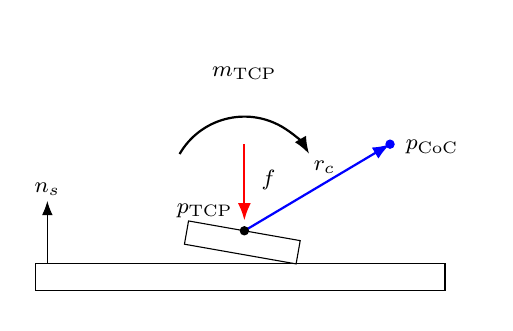
\begin{tikzpicture}[
 font=\small,
 surf/.style={draw=black,fill=white},
 tool/.style={draw=black,fill=white},
 frc/.style={-{Latex[length=2.2mm]},thick,red},
 lev/.style={-{Latex[length=2.2mm]},thick,blue},
 mom/.style={-{Latex[length=2.2mm]},thick,black},
 ax/.style={-{Latex[length=1.8mm]},black},
 lbl/.style={font=\footnotesize,inner sep=1.8pt},
 pt/.style={circle,fill=black,inner sep=0pt,minimum size=3.4pt},
 cpt/.style={circle,fill=blue,inner sep=0pt,minimum size=3.4pt}]
\useasboundingbox (-2.7,-0.50) rectangle (3.1,3.0);
\fill[surf] (-2.6,-0.34) rectangle (2.6,0);
\draw[black] (-2.6,0)--(2.6,0);
\draw[ax] (-2.45,0)--(-2.45,0.80) node[lbl,above] {$n_s$};
\begin{scope}[shift={(0,0.125)},rotate=-10]
 \draw[tool] (-0.72,0) rectangle (0.72,0.30);
 \coordinate (T) at (0,0.30);
\end{scope}
\coordinate (P) at ($(T)+(1.85,1.10)$);
\draw[lev] (T)--(P);
\node[lbl,above,black] at ($(T)!0.55!(P)+(0,0.05)$) {$r_c$};
\node[pt] at (T) {};
\node[lbl,anchor=south east] at ($(T)+(-0.08,0.10)$) {$p_{\mathrm{TCP}}$};
\node[cpt] at (P) {};
\node[lbl,anchor=west] at ($(P)+(0.13,-0.04)$) {$p_{\mathrm{CoC}}$};
\draw[frc] ($(T)+(0,1.10)$)--($(T)+(0,0.13)$);
\node[lbl,right,black] at ($(T)+(0.15,0.65)$) {$f$};
\coordinate (M) at ($(T)+(0,0.50)$);
\draw[mom] ([shift=(150:0.95)]M) arc (150:30:0.95);
\node[lbl] at ($(T)+(0,2.00)$) {$m_{\mathrm{TCP}}$};
\end{tikzpicture}
\end{document}
